\documentclass[12pt]{report}

%%%%%%%%%%%%%%%%%%%%%%%%%%%%%%%%%%%%%%%%%%%%%%%%%%%%%%%%

%%% General Packages
\usepackage{amsmath, amssymb, amsthm}
\usepackage{titling}
\usepackage{titlesec}
\usepackage{geometry}
\usepackage{enumerate}

\usepackage[hidelinks]{hyperref}



%%% Font and Text Packages
%\usepackage{newpxtext}
%\usepackage{newpxmath}

\usepackage[sc]{mathpazo}
\usepackage{avant}

\usepackage[dvipsnames]{xcolor}


%%% Graphics, Figure and Listing Packages
\usepackage{graphicx}
\usepackage{xcolor}
\usepackage{float}
\usepackage{calc}
\usepackage{caption}
\usepackage{subcaption}
\usepackage[framemethod=tikz]{mdframed}


%%% Epigraph
\usepackage{epigraph}

%%% Bibliography Packages
\usepackage[style=alphabetic]{biblatex}
\bibliography{references}

%%%%%%%%%%%%%%%%%%%%%%%%%%%%%%%%%%%%%%%%%%%%%%%%%%%%%%%%

%%% Page Formatting Options
\geometry{left = 2.5cm}
\geometry{right = 2.5cm}
\geometry{top = 2.5cm}
\geometry{bottom = 2.5cm}

%%% Section and Chapter Titling Options

\titleformat{\chapter}[display]
{\normalfont\bfseries\LARGE}
{\chaptertitlename~\thechapter}
{0pc}
{{\color{black!30!white}\titlerule[2pt]}\vspace{0.8pc}\normalfont\Large}

\titleformat{name=\chapter, numberless}[display]
{\normalfont\bfseries\LARGE}{}{1pc}
{\normalfont\Large}

\titlespacing*{\chapter}{0pt}{30pt}{40pt}

\titleformat{\section}
{\normalfont\bfseries\large}
{\normalfont\bfseries\large{\thesection}}
{1em}
{}

%%% Hyperlink Formatting Options
\hypersetup{
        colorlinks,
        linkcolor={black},
        citecolor={blue!60!black},
        urlcolor={blue!80!black}
}

%%% Epigraph Options and Setup
\setlength\epigraphwidth{0.6\textwidth}
\setlength{\epigraphrule}{0pt}


%%%%%%%%%%%%%%%%%%%%%%%%%%%%%%%%%%%%%%%%%%%%%%%%%%%%%%%%

%%% Graphics and Figure Options
% Graphics path (necessary for .svg images).
\graphicspath{{graphics/}}
\counterwithout{figure}{chapter}
\counterwithout{table}{chapter}

% Caption setup
\captionsetup{margin=1.5cm}

%%%%%%%%%%%%%%%%%%%%%%%%%%%%%%%%%%%%%%%%%%%%%%%%%%%%%%%%

%%% Palettes

%%%%%%%%%%%%%%%%%%%%%%%%%%%%%%%%%%%%%%%%%%%%%%%%%%%%%%%%


%%% Personal Macros
\newcommand{\N}{\mathbb{N}}
\newcommand{\R}{\mathbb{R}}
\newcommand{\Z}{\mathbb{Z}}
\newcommand{\T}{\mathbb{T}}
\renewcommand{\S}{\mathbb{S}}
\newcommand{\ip}[2]{\langle #1, #2 \rangle}
\newcommand{\inject}{\lhook\joinrel\longrightarrow}

\newcommand{\kob}{\operatorname{kob}}
\newcommand{\lk}{\operatorname{\ell\textit{k}}}

\newcommand{\hash}{\ensuremath{\mathbin{\#}}}
\renewcommand{\over}{\text{O}}
\newcommand{\under}{\text{U}}

%%% amsthm Environments

% Define mdf style
\mdfdefinestyle{lined}{%
        middlelinewidth=2pt,
        middlelinecolor=black,
        bottomline=false,topline=false,rightline=false,
        innertopmargin=-3pt
}

\newtheoremstyle{regular}% name
  {}%         Space above, empty
  {}%         Space below
  {\upshape}% Body font
  {}%         Indent amount (empty = no indent, \parindent = para indent)
  {\bfseries\scshape}% Thm head font
  {.}%        Punctuation after thm head
  {.7em}% Space after thm head: \newline = linebreak
  {}%         Thm head spec

\theoremstyle{regular}

\newtheorem{thm}{Theorem}

\newtheorem{theorem}{Theorem}
\surroundwithmdframed[style=lined,middlelinecolor=PineGreen]{theorem}

\newtheorem{example}{Example}
\surroundwithmdframed[style=lined,middlelinecolor=PineGreen]{example}

\newtheorem{definition}{Definition}
\surroundwithmdframed[style=lined,middlelinecolor=RubineRed]{definition}

\newtheorem{proposition}{Proposition}
\surroundwithmdframed[style=lined,middlelinecolor=Plum]{proposition}

\newtheorem{conjecture}{Conjecture}
\surroundwithmdframed[style=lined,middlelinecolor=BrickRed]{conjecture}

\newtheorem{lemma}{Lemma}
\surroundwithmdframed[style=lined,middlelinecolor=Aquamarine]{lemma}

\newtheorem{corollary}{Corollary}
\surroundwithmdframed[style=lined,middlelinecolor=RoyalPurple]{corollary}

%%% Drafting Macros

\mdfdefinestyle{draftnote}{%
        outerlinewidth=0.4pt,
        innerlinewidth=0.4pt,
        middlelinewidth=1pt,
        middlelinecolor=white,
        backgroundcolor=red!15,
}
\newcommand{\draftnote}[1]{
\begin{mdframed}[style=draftnote]
        {\color{Gray}{\scshape Note:} #1 }
\end{mdframed}
}


\mdfdefinestyle{scaffold}{%
        outerlinewidth=0.4pt,
        innerlinewidth=0.4pt,
        middlelinewidth=1pt,
        middlelinecolor=white,
        backgroundcolor=lightgray!60,
}
\newcommand{\scaffold}[1]{
\begin{mdframed}[style=scaffold]
        {\color{teal}#1}
\end{mdframed}
}

\newcommand{\red}[1]{
        {\color{BrickRed}#1}
}


%%%%%%%%%%%%%%%%%%%%%%%%%%%%%%%%%%%%%%%%%%%%%%%%%%%%%%%%

\begin{document}

        %%% Make titlepage.

        % Titlepage Options
        \author{Damian Lin}
        \title{(Towards) A Unified Topological Kashiwara-Vergne Theory}

        \cleardoublepage \thispagestyle{empty}
        \null \vfil
        \begingroup
        \LARGE \bfseries \centering
        \openup \medskipamount
        \thetitle \par \vspace{30pt}
        \centering \mdseries \theauthor \par \bigskip
        \endgroup
        \vfil \vfil \vfil
        \begin{center}
                An essay submitted in partial fulfilment of\\
                the requirements for the degree of\\
                Master of Philosophy (Science)
                \vfil\vfil
                {\large Pure Mathematics\\[5pt]
                        University of Sydney}\\
                \vskip6mm
                
\includegraphics[width=25mm]{graphics/USY_MB1_CMYK_Stacked_Logo.pdf}
                \vfil
                \normalsize\today
        \end{center}
        \vfil
        \cleardoublepage

        \tableofcontents

        \chapter*{Acknowledgements}
        \addcontentsline{toc}{chapter}{Acknowledgements}

        These are the acknowledgements.

        \chapter*{Introduction}
        \addcontentsline{toc}{chapter}{Introduction}

        \section*{The Idea of Finite Type Invariants}
        \draftnote{Here I want to motivate the study of Finite-type invariants in general, using analogies from discriminant theory.}

        The essence of singularity theory, developed by Arnold, Thom, Vassiliev, etc. is that various geometric or topological objects can be studied by considering not only those objects, but also their singular versions, and using this `discriminant set' to define and compute invariants. Take for example the following simple analogy, from \cite{knots-links-and-their-invariants}.

        In this analogy, instead of studying some topological object (say, the space of knots), we study a much simpler geometric one: the space of quadratic equations without multiple roots. For now, let us have real coefficients and real roots.

        \begin{example}[Quadratic equations with real roots]
                All quadratic equations can be put in the form \(x^{2} + px + q = 0\), and then represented as a point in the \((p, q)\) coordinate plane. By completing the square, those quadratic equations with one root which we ignored live on the parabola \(P\) given by \(q = p^{2}/4\).

                The number of roots of each point \((p, q)\) can then be calculated as follows. First, choose a starting point, say \((1, 0)\) which represents \(x^{2} + x = 0\), having two roots. Choose also a curve \(C\) in general position with respect to \(P\), from \((1, 0)\) to \((p, q)\). Put an orientation on the curve traced out by the parabola \(P\), such as below. Then, starting at \((1, 0)\) and traversing along the curve, note that every time the \(C\) intersects \(P\) `negatively', the number of roots decreases by two, and a `positive` intersection increases the number of roots by two.

                \begin{figure}[H]
                        \centering
                        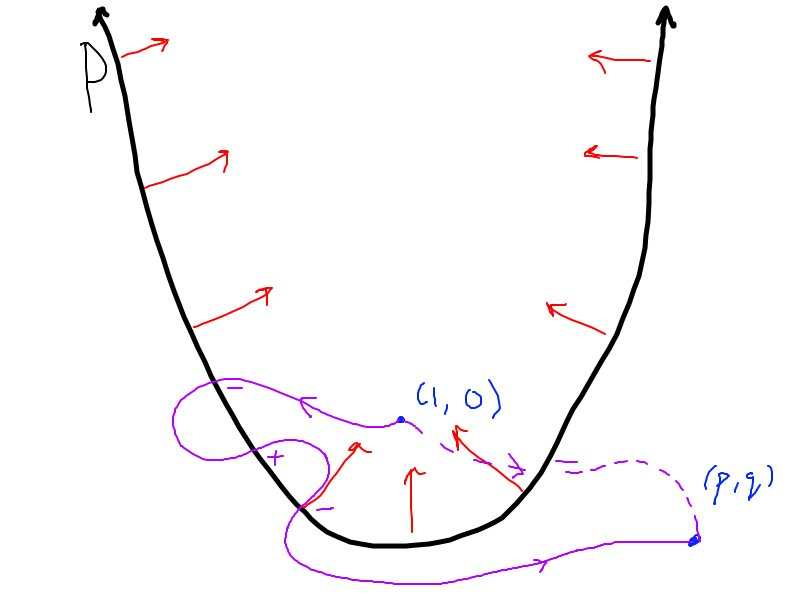
\includegraphics[width=0.4\textwidth]{graphics/parabola_example.jpg}
                \end{figure}

                The function \(R(p, q)\) that sends a quadratic equation to its number of roots is an invariant of the nice `space' of all quadratic equations with the singular locus \(P\) removed. But the moral of the story is that certain nice invariants of the `nice' space can be constructed by considering the `ugly' space that includes some `discriminant set' (in this case \(P\)), by setting the invariant, say \(f\) to take some value on \(P\), and enforcing that the value of the invariant changes by \(\pm f(P)\) on any path crossing through \(P\), depending on orientation. One could write this rule as

        \begin{figure}[H]
                \centering
                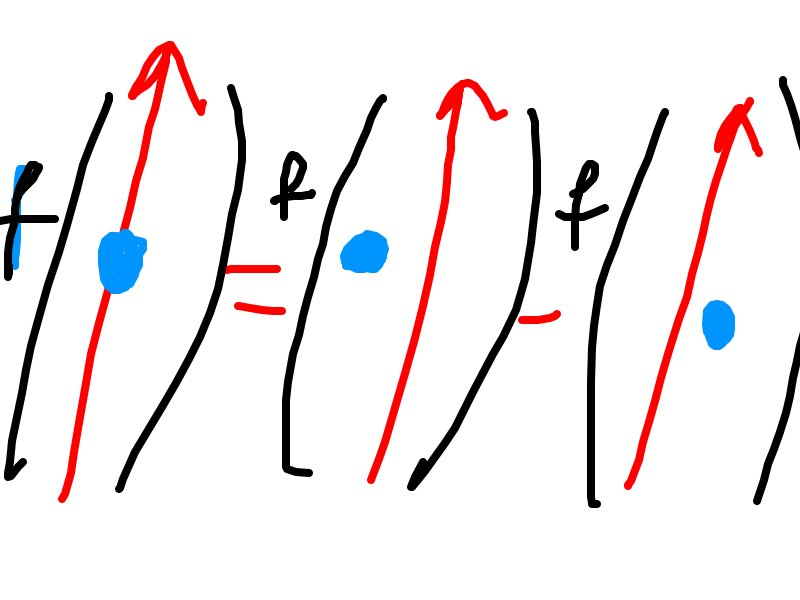
\includegraphics[width=0.3\textwidth]{graphics/simple_singularity_relation.jpg}
        \end{figure}
        \end{example}



        \section*{Finite Type Invariants of Knots}

        Let's translate this idea into knot theory, following the work of Vassiliev in \cite{cohomology-of-knot-spaces, complements-of-discriminants-of-smooth-maps-topology-and-applications}. The generic objects of study in knot theory are smooth embeddings \(S^{1} \hookrightarrow \R^{3}\). A \textit{knot} can either mean an equivalence class of such embeddings up to ambient isotopy, or a specific embedding, depending on the context.

        The space of knots, that is the configuration space of all smooth embeddings, lies within the space of all smooth maps \(S^{1} \to \R^{3}\) (which we denote \(K\)). And the discriminant space \(\Sigma\) is the space of all maps with singularities or self-intersections. The discriminant space is `stratified' into the components by subspaces of smooth maps with multiple self-intersections; the space with \(i\) such singularities we call \(\Sigma_{i}\).

        Then, each knot corresponds to a component of \(K \smallsetminus \Sigma\), and numerical invariants of knots correspond to elements of \(H^{0}(K \smallsetminus \Sigma)\).
        \draftnote{
                My intention here is to convince the reader that finite type invariants and chord diagrams are important by fleshing out the above analogy. I want to expand the above paragraph to include:
                \begin{itemize}
                        \item If \(H^{0}(K \smallsetminus \Sigma)\) are all knot invariants, in terms of cohomology, what are the finite type invariants?
                        \item Are the above defined in terms of invariants (functions) \(H^{0}(K \smallsetminus \Sigma_{i})\) (defined on higher levels of the stratification)?
                        \item What are the interpretations of \(H^{i}(K \smallsetminus \Sigma)\) \cite[p.149]{complements-of-discriminants-of-smooth-maps-topology-and-applications}?
                        \item According to Sossinsky in \cite[p. 49]{knots-mathematics-with-a-twist} Vassiliev's work (presumably in \cite{complements-of-discriminants-of-smooth-maps-topology-and-applications, cohomology-of-knot-spaces}) says that different paths through \(K\), amounting to different calculations of a finite type invariant, give the same result. What, precisely, is this statement in terms of homology/cohomology?
                        \item Maybe but also maybe not yet: How do chord diagrams come into this? (I think they determine how the higher levels of the stratification can take on different values under finite type invariants).
                \end{itemize}

                Something like:
        }

        The work of Vassiliev is to understand the space
        \(K \smallsetminus \Sigma\).
        Paths through this space correspond to isotopy on knots, so each component corresponds to a different knot. The locally constant functions on this space, that is the zeroth cohomology group,
        \({H^{0}(K \smallsetminus \Sigma, \mathcal{R})}\)
        is exactly the group of knot invariants valued in
        \(\mathcal{R}\).

        % TODO: Get someone who has any idea about spectral sequences to read this and see if it makes sense
        In fact, Vassiliev looks at the more general question of computing the cohomology ring
        \({H^{\ast}(K \smallsetminus \Sigma, \mathcal{R}})\).
        The Vassiliev invariants (of order \(i\)) are a certain subgroup of
        \({H^{0}(K \smallsetminus \Sigma)}\)
        that (roughly) can be written as linking numbers with cycles in the homology group of the strata at depth \(i\) of the discriminant, cycles in
        \({H_{n - 1}(\Sigma_{i}, \mathcal{R})}\).

        As summarised in \cite{introduction-to-vassiliev-invariants}, Vassiliev constructs and uses tools in the arsenal of singularity theory to compute terms of the cohomological spectral sequence \(E^{p, q}_{r}\), and while it is unclear whether this contains all of the cohomological information about \({K \smallsetminus \Sigma}\), its zero-dimensional cohomology classes are exactly the Vassiliev invariants.

        In a more down-to-earth way of putting it, Vassiliev invariants are those which differ by predictable amounts on different sides of the strata, that is obeying the relation
        \begin{figure}[H]
                \centering
                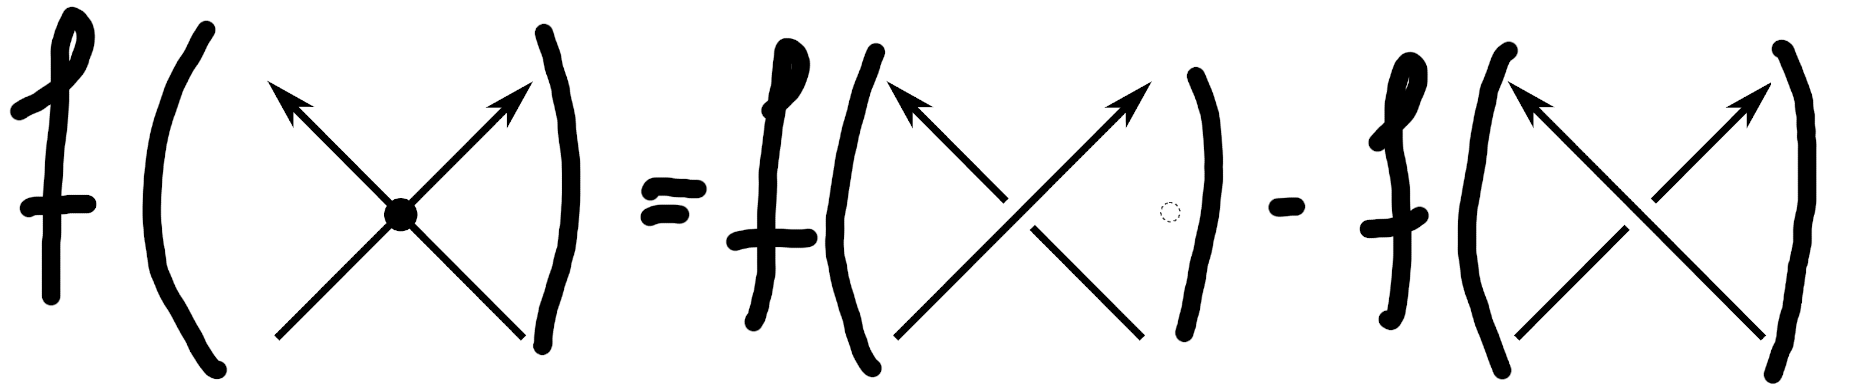
\includegraphics[width=0.3\textwidth]{graphics/vassiliev_relation.png}
        \end{figure}
        \noindent
        in which after some depth in the strata, the left hand side of the above is always zero, meaning that \(f\) is unchanged by that part of the strata.

        Invariants of Vassiliev's type are determined (up to lower order Vassiliev invariants) by \textit{weight systems} or equivalently, by their values on the the dual space of \textit{chord diagrams}. In Chapter \ref{ch:formality-and-chord-diagrams} we will approach Vassiliev invariants from this angle: by focussing instead on the algebra of chord diagrams, the associated graded space of knots. We discuss an algebraic construction of the Universal Vassiliev Invariant due to Drinfeld which makes the link to quantum algebra.

        In Chapter \ref{ch:lie-theory-and-jocobi-diagrams}, we find an isomorphism between the algebra of chord diagrams and the algebra of Jacobi diagrams. It becomes clear that Lie theory is the proper way to view this algebra and others like it.

        \scaffold{In chapter \(X\) we will talk about \(Y\).}

        \chapter{Formality and Chord Diagrams}
        \label{ch:formality-and-chord-diagrams}

        \scaffold{Filtered structures, associated graded structures, formality and how this leads to conections between Vassiliev Invariants and quantum algebra via a general application of Von Dyck's Theorem. Can include intro to PaT Vassiliev filatration, chord diagrams, Drinfeld Associators on a story sort of level.}


        \scaffold{In more detail. A section will be on chord diagrams and the associated graded. Since the introduction comes from the Vassiliev history space-of-knots point-of-view, I want to do things pretty formally with respect to the associated graded space. i.e. I don't want to say double point = overcrossing - undercrossing, as these two things are definitely not equal, but it is okay to say V(d.p.) = V(over) - V(under). To do this requires the treatment in \cite{the-fundamental-theorem-of-vassiliev-invariants}, which on the bright side means I get to talk about the polynomials analogy. It means that the statement becomes \[\text{weight systems} = \operatorname{gr}(\text{Vassiliev invariants})\] instead of directly \[\text{chord diagrams} = \operatorname{gr}(\text{singular knots})\] (or at least that's how it's put in \cite{the-fundamental-theorem-of-vassiliev-invariants}, but perhaps this can also be turned into a statement without all the implicit duals.}


        %\section{Filtrations}
        %\section{Associated Graded Functor}
        %\section{Finite Type Invariants and Chord Diagrams}

        \chapter{Lie Theory and Jacobi Diagrams}
        \label{ch:lie-theory-and-jocobi-diagrams}

        \section{(Rooted) Jacobi Diagrams}

        \section{Floating Jacobi Diagrams}

        \scaffold{In the next section we construct the suprising isomorphism between these two spaces.}

        \section{PBW Theorem}

        \scaffold{The Poincare-Birkhoff-Witt theorem for Lie algebras has many forms. One of these is that [...] . A corollary of this theorem \cite{enveloping-algebras} is that there is a `canonical' (though, not natural) isomorphism \(S(\mathfrak{g}) \to \mathcal{U}(\mathfrak{g})\) given by \[\omega(x_{1} \cdots x_{n}) = \frac{1}{n!} \sum_{\sigma \in S_{n}} x_{\sigma(1)} \cdots x_{\sigma(n)}.\] Which simply exhibits that fact that \(\operatorname{gr} A \cong A\) unnaturally.}

        \scaffold{Futher, \cite{enveloping-algebras}, the two spaces (though not isomorphic as algebras) are isomorphic as \(\mathfrak{g}\)-modules: \(\mathcal{U}(\mathfrak{g})^{\mathfrak{g}} \cong S(\mathfrak{g})^{\mathfrak{g}}\).}

        \scaffold{The following theorem is a diagrammatic version of the above.}

        \chapter{Welded Knots, Foams and the Kashiwara-Vergne Equations}

        \chapter{Existing Topological Interpretations of the Kashiwara-Vergne Equations}

        \section{Lie Theory}

        \section{Goldman-Turaev}

        \section{Welded Foams}

        \chapter{Topological Approaches}
        \scaffold{Welded foams (WKOII) vs Goldman-Turaev (AKKN) - pointing out the differences.}

        \draftnote{Would be good to try writing here.}

        \chapter{Emergent Tangles: Lifting Goldman-Turaev to 3 Dimensions}
        \scaffold{Paper of Zsuzsi, Dror, Nancy, Jessica, Tamara.}

        \chapter{Emergent w-foams: Lifting Goldman-Turaev to 4 Dimensions}
        \draftnote{The content of this chapter is mathematics that still needs to be done.}

        \chapter{Virtual Knot Tabulation (if present)}

        \appendix
        \titleformat{\chapter}[display]
        {\normalfont\bfseries\LARGE}
        {\chaptertitlename~\thechapter}
        {0pc}
        {{\color{black!30!white}\titlerule[0.7pt]}{\color{white}\titlerule[0.7pt]}{\color{black!30!white}\titlerule[0.7pt]}\vspace{0.8pc}\normalfont\Large}

        % \chapter{appendixname}
        % This is the first appendix.


        \newpage
        \printbibliography[title=References]


\end{document}
